\documentclass[aspectratio=169]{beamer}

\usepackage[utf8]{inputenc}
\usepackage{graphicx}
\usepackage{tikz}
\usetikzlibrary{positioning, arrows.meta, calc}
\usepackage{fontawesome5}

\usefonttheme{professionalfonts}

\usetheme{Madrid}
\definecolor{slideblue}{RGB}{100, 160, 210}
\definecolor{ucdgreen}{RGB}{0, 102, 51}
\definecolor{drybrown}{RGB}{180, 120, 40}
\definecolor{wetblue}{RGB}{30, 100, 180}
\definecolor{darkink}{RGB}{14, 42, 61}
\definecolor{naored}{RGB}{180, 50, 50}
\usecolortheme[named=wetblue]{structure}
\setbeamertemplate{navigation symbols}{}
\setbeamersize{text margin left=7mm, text margin right=7mm}
\setbeamertemplate{headline}{}
\setbeamercolor{upper separation line foot}{bg=white}
\setbeamercolor{middle separation line foot}{bg=white}
\setbeamercolor{lower separation line foot}{bg=white}
\setbeamercolor{author in head/foot}{fg=wetblue!70!black, bg=wetblue!10}
\setbeamercolor{title in head/foot}{fg=wetblue!70!black, bg=wetblue!10}
\setbeamercolor{date in head/foot}{fg=wetblue!70!black, bg=wetblue!10}
\setbeamertemplate{footline}{%
  \leavevmode%
  \hbox{%
    \begin{beamercolorbox}[wd=.333333\paperwidth,ht=2.25ex,dp=1.5ex,center]{author in head/foot}%
      \usebeamerfont{author in head/foot}\insertshortauthor
    \end{beamercolorbox}%
    \begin{beamercolorbox}[wd=.333333\paperwidth,ht=2.25ex,dp=1.5ex,center]{title in head/foot}%
      \usebeamerfont{title in head/foot}\insertshorttitle
    \end{beamercolorbox}%
    \begin{beamercolorbox}[wd=.333333\paperwidth,ht=2.25ex,dp=1.5ex,right]{date in head/foot}%
      \usebeamerfont{date in head/foot}%
      \insertframenumber{} / \inserttotalframenumber\hspace*{2ex}
    \end{beamercolorbox}}%
  \vskip0pt%
}

\title[Journal Club $\cdot$ 06 May 2026]{Journal Club}
\author[Lainey Ward]{Lainey Ward}
\institute[]{}
\date{}

\begin{document}

% SLIDE 1: Title
\begin{frame}

\begin{columns}[T]
    \begin{column}{0.60\textwidth}
        \vspace{2.0cm}

        {\large\bfseries\color{darkink}
         Abrupt Drought Termination in the
         British--Irish Isles Driven by High
         Atmospheric Vapour Transport}

        \vspace{1.5em}
        \textcolor{gray!50}{\rule{3cm}{0.5pt}}

        \vspace{0.5em}
        {\small\color{gray}
         Parry et al.\ (2023),
         \textit{Environmental Research Letters}}

    \end{column}

    \begin{column}{0.40\textwidth}
        \vspace{0.5cm}
        
\begin{tikzpicture}
            \fill[drybrown!40] (0,0) rectangle (4.5,3.2);
            \fill[wetblue!40] (0,3.2) rectangle (4.5,6.4);
        \end{tikzpicture}
    \end{column}
\end{columns}

\end{frame}

% SLIDE 2: What's the Hypothesis?
\begin{frame}{What's the Hypothesis?}

\begin{columns}[c]
    \begin{column}{0.48\textwidth}
        \begin{center}
            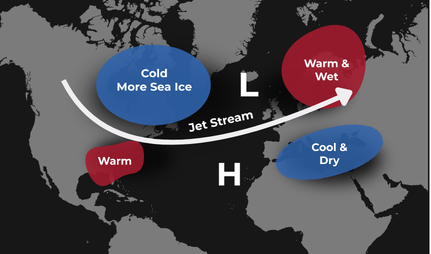
\includegraphics[width=0.88\textwidth]{nao_positive.png}

            \vspace{0.3em}
            {\scriptsize\color{gray} Adapted from Climate Data Canada}
        \end{center}
    \end{column}

    \begin{column}{0.52\textwidth}

        {\footnotesize\color{gray} 01}\quad
        {\normalsize\bfseries\color{darkink} \textcolor{naored}{NAO+} shifts jet stream over Ireland}

        \vspace{1.2em}
        \textcolor{gray!30}{\rule{\textwidth}{0.4pt}}
        \vspace{0.3em}

        {\footnotesize\color{gray} 02}\quad
        {\normalsize\bfseries\color{darkink} \textcolor{wetblue}{Atmospheric rivers} carry moisture}

        \vspace{1.2em}
        \textcolor{gray!30}{\rule{\textwidth}{0.4pt}}
        \vspace{0.3em}

        {\footnotesize\color{gray} 03}\quad
        {\normalsize\bfseries\color{darkink} \textcolor{ucdgreen}{Uplift} $\rightarrow$ heavy rainfall}

    \end{column}
\end{columns}

\end{frame}

% SLIDE 3: How Did They Test It?
\begin{frame}{How Did They Test It?}

\begin{center}
    \begin{tikzpicture}

        % Data source 1: Simulated flows (top left) — green for hydrology
        \node[draw=ucdgreen, thick, rounded corners=8pt,
              minimum width=2.6cm, minimum height=1.7cm,
              fill=ucdgreen!8] (s1) at (0,5.8) {};
        \node[font=\Large, ucdgreen] at (0,6.2) {\faWater};
        \node[font=\bfseries\footnotesize, ucdgreen!90!black] at (0,5.4) {Simulated flows};

        % DT events (top middle) — green for hydrology
        \node[draw=ucdgreen, thick, rounded corners=8pt,
              minimum width=2.6cm, minimum height=1.7cm,
              fill=ucdgreen!8] (s2) at (3.8,5.8) {};
        \node[font=\Large, ucdgreen] at (3.8,6.2) {\faCalendarCheck};
        \node[font=\bfseries\footnotesize, ucdgreen!90!black] at (3.8,5.4) {DT events};

        % Data source 2: ERA-20C IVT (bottom left) — blue for atmosphere
        \node[draw=wetblue, thick, rounded corners=8pt,
              minimum width=2.6cm, minimum height=1.7cm,
              fill=wetblue!8] (s3) at (0,3.0) {};
        \node[font=\Large, wetblue] at (0,3.4) {\faCloudRain};
        \node[font=\bfseries\footnotesize, wetblue] at (0,2.6) {ERA-20C IVT};

        % Binary series box
        \node[draw=darkink, thick, rounded corners=8pt,
              minimum width=5.2cm, minimum height=3.6cm,
              fill=darkink!5] (s4) at (8.5,4.4) {};

        \node[font=\bfseries\footnotesize, darkink] at (8.5,5.8) {Binary series};

        % Row 1: DT binary (green 1s match hydrology boxes)
        \node[font=\large, anchor=west] at (6.4,4.9)
            {\texttt{0~0~0~}%
             {\bfseries\color{ucdgreen}1}%
             \texttt{~0~0~0}};

        % Divider
        \draw[gray!30, thick] (6.2,4.3) -- (10.8,4.3);

        % Row 2: IVT binary (blue 1s match atmosphere box)
        \node[font=\large, anchor=west] at (6.4,3.7)
            {\texttt{0~}%
             {\bfseries\color{wetblue}1}%
             \texttt{~}%
             {\bfseries\color{wetblue}1}%
             \texttt{~0~0~0~0}};

        % Arrows
        \draw[-{Stealth[length=3mm]}, thick, ucdgreen!60] (s1) -- (s2);
        \draw[-{Stealth[length=3mm]}, thick, ucdgreen!60] (s2) -- (s4);
        \draw[-{Stealth[length=3mm]}, thick, wetblue!60] (s3) -- (s4);

    \end{tikzpicture}
\end{center}

\end{frame}

% SLIDE 4: What Did They Find?
\begin{frame}{What Did They Find?}

\begin{columns}[c]
    \begin{column}{0.40\textwidth}

        {\normalsize\bfseries\color{wetblue} 53\%} {\normalsize\bfseries\color{darkink} preceded by high IVT}

        \vspace{1.2em}
        \textcolor{gray!30}{\rule{\textwidth}{0.4pt}}
        \vspace{0.3em}

        {\normalsize\bfseries\color{darkink} Most abrupt: \textcolor{naored}{NAO+} + \textcolor{wetblue}{IVT}}

        \vspace{1.2em}
        \textcolor{gray!30}{\rule{\textwidth}{0.4pt}}
        \vspace{0.3em}

        \raisebox{-0.4em}{
\includegraphics[height=1.4em,keepaspectratio]{ireland_icon.png}}\;
        {\normalsize\bfseries\color{darkink} year-round}

    \end{column}

    \begin{column}{0.60\textwidth}
        \begin{center}
            \begin{tikzpicture}
                \node[inner sep=0pt] (plot) {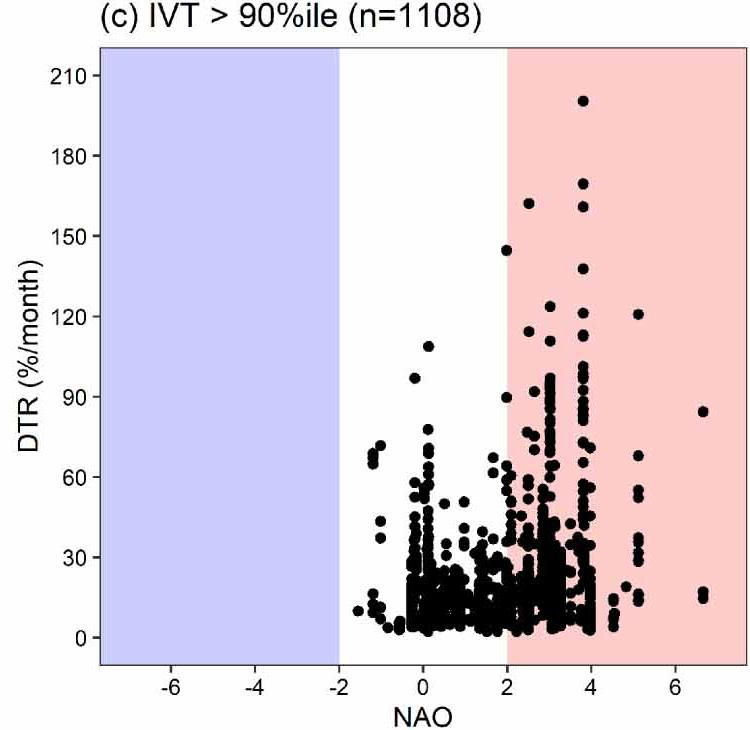
\includegraphics[width=0.82\textwidth]{fig4c_only.jpg}};
                % Circle: DTR > ~120, NAO 2-5 (most abrupt terminations)
                \draw[naored, very thick]
                    (1.9,1.5) ellipse (1.1cm and 1.3cm);
            \end{tikzpicture}
        \end{center}
    \end{column}
\end{columns}

\end{frame}

% SLIDE 5: Conclusion
\begin{frame}{Conclusion}

\vfill
\begin{center}
    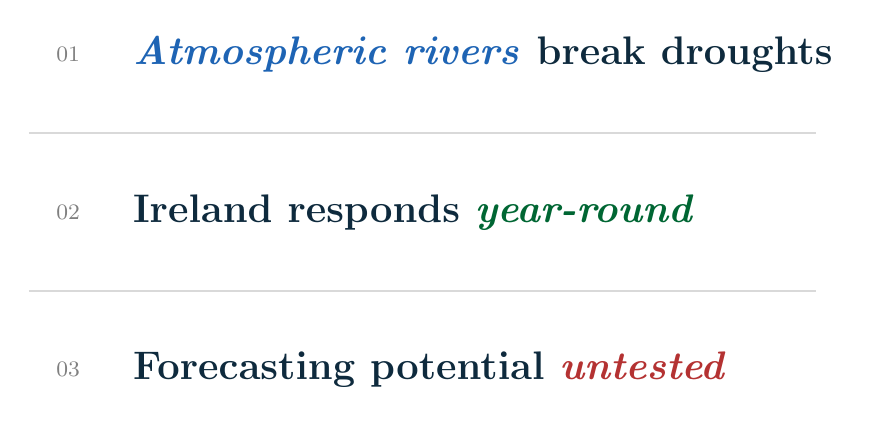
\begin{tikzpicture}

        % Line 1
        \node[font=\footnotesize, gray] at (-4.5,2.0) {01};
        \node[font=\Large\bfseries, darkink, anchor=west] at (-3.8,2.0)
            {\color{wetblue}\textit{Atmospheric rivers} \color{darkink}break droughts};

        % Line 2
        \draw[gray!30, thick] (-5,1.0) -- (5,1.0);
        \node[font=\footnotesize, gray] at (-4.5,0.0) {02};
        \node[font=\Large\bfseries, darkink, anchor=west] at (-3.8,0.0)
            {Ireland responds \color{ucdgreen}\textit{year-round}};

        % Line 3
        \draw[gray!30, thick] (-5,-1.0) -- (5,-1.0);
        \node[font=\footnotesize, gray] at (-4.5,-2.0) {03};
        \node[font=\Large\bfseries, darkink, anchor=west] at (-3.8,-2.0)
            {Forecasting potential \color{naored}\textit{untested}};

    \end{tikzpicture}
\end{center}
\vfill

\end{frame}

\end{document}
